\documentclass[conference]{IEEEtran}
\usepackage[T1]{fontenc}
\usepackage{cite}
\usepackage{amsmath,amssymb}
\usepackage{booktabs}
\usepackage{multirow}
\usepackage{xcolor}
\usepackage{url}
\usepackage{graphicx}
\usepackage{tikz}
\usetikzlibrary{positioning,arrows.meta,fit,calc,backgrounds}
\usepackage{array}
\usepackage[hidelinks]{hyperref}

% Marks numbers that come from runs still in progress; must be empty before submission.
\newcommand{\pending}[1]{\textcolor{red}{\textsf{[PENDING: #1]}}}

\setlength{\tabcolsep}{4pt}
\begin{document}

\title{Air-HUIM: Exact High-Utility Itemset Mining\\Under a Hard Memory Budget on Edge Hardware}

\author{\IEEEauthorblockN{Arya Gupta}
\IEEEauthorblockA{\textit{Department of Computer Science and Engineering}\\
\textit{University of Engineering and Management}\\
Kolkata, India\\
aryagupta.dev@gmail.com}}

\maketitle

\begin{abstract}
High-utility itemset mining (HUIM) finds sets of items whose combined value, such as profit,
exceeds a threshold. Its algorithms are designed and evaluated on desktops and servers with
16--128\,GB of memory, and the reference implementations report memory use but never bound it.
We present Air-HUIM, a Rust library of 23 HUIM algorithms that run exactly under a
user-set memory budget. One memory ledger accounts for every structure that grows with the data;
each algorithm spills, recomputes or partitions its state when the budget is reached, and refuses
up front when the budget is below a computed minimum. The unifying idea is that the location of search
state never changes the result: state can be spilled, recomputed from its parents, avoided by
partitioning the search, or relaxed to a looser valid bound, and memory pressure costs time,
never answers. On a 4\,GB Raspberry
Pi~4, across 14 datasets and budgets from 24\,MB to 2\,GB, no Air-HUIM run was killed for
memory, all 905 runs with a reference output were exact, and a kernel-enforced limit killed no
Air-HUIM run. At the same budgets, the reference Java library SPMF ran out of memory in 229 of
588 runs. Air-HUIM mines the 47.1-million-basket dunnhumby LGSR dataset on the Pi within 1 and
2\,GB, where SPMF fails in all 8 runs. Verifying every disagreement by a full scan also revealed
three correctness bugs in SPMF.
\end{abstract}

\begin{IEEEkeywords}
high-utility itemset mining, memory-bounded algorithms, edge computing, Raspberry Pi, Rust
\end{IEEEkeywords}

% ---------------------------------------------------------------------------------------------
\section{Introduction}

High-utility itemset mining generalises frequent itemset mining: each item in a transaction
carries a quantity and a unit value, and the task is to find every itemset whose total utility
in the database reaches a threshold \texttt{min\_util}~\cite{twophase2005,survey2019}. Retail
analysis is the standard application: which products together bring in the most revenue.

Two decades of work have made HUIM algorithms much faster~\cite{huiminer2012,fhm2014,efim2017,upgrowth2013}.
They have been evaluated almost exclusively on well-provisioned machines. The standard empirical
comparison~\cite{zhang2018} ran SPMF~\cite{spmf2016}, the reference implementation of most of
these algorithms, on a 4.4\,GHz desktop with 128\,GB of RAM and a 128\,GB Java heap. Memory is
reported as an outcome of a run, never as a constraint on it. Parallel work targets 96-thread
servers~\cite{dphim2026} and GPUs~\cite{gahuim2026}.

This leaves a practical question open: can these algorithms run \emph{exactly} on the hardware
where much retail and sensor data is produced, such as a single-board computer with a few
gigabytes of RAM, without the analyst having to guess whether a run will fit? On a 4\,GB
Raspberry Pi, SPMF fails on 47.1\,million baskets at every budget we tried, and on the classic
benchmark datasets it runs out of memory at a 64\,MB heap in 116 of 196 runs
(Section~\ref{sec:eval}). Fig.~\ref{fig:trace} shows the difference on one run.

\begin{figure}[t]
\centering
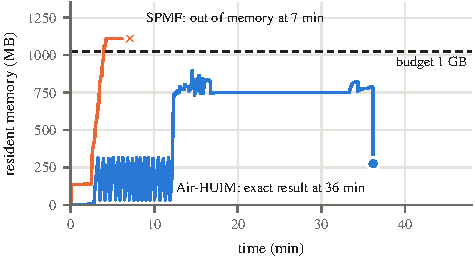
\includegraphics[width=\columnwidth]{fig/trace_lgsr.pdf}
\caption{Resident memory over time, FHM on 47.1\,M baskets (LGSR) with a 1\,GB budget on a 4\,GB
Raspberry Pi. SPMF grows until the JVM runs out of memory; Air-HUIM stays under the budget and
returns the exact result. The oscillation before minute 12 is the external sort that builds the
1-itemset lists, spilling and refilling its buffer.}
\label{fig:trace}
\end{figure}

We present \textbf{Air-HUIM}, a Rust library in which the memory budget is a first-class input.
The user gives one number; every algorithm keeps the process within it, uses the memory it is
given, and returns exactly the same itemsets at every budget. Our contributions are:
\begin{enumerate}
\item \textbf{Budgeted state, one idea for 23 algorithms} (Section~\ref{sec:idea}): four moves on
search state (spill, recompute, partition, relax) that provably preserve the output, a resident
core below which a run refuses, and an operator matrix that gives every algorithm's memory model.
\item \textbf{An architecture that executes the moves} (Section~\ref{sec:design}): engines reserve
every growing structure from one state manager (ledger, move policy, admission control, RSS
feedback) that shares its budget with the buffer pool.
\item \textbf{An evaluation on a 4\,GB Raspberry Pi} (Section~\ref{sec:eval}): 1,503 runs over
14 datasets and budgets from 24\,MB to 2\,GB, against SPMF at the same budgets and under a
kernel-enforced memory limit, plus a 47.1-million-basket retail dataset.
\item \textbf{Three correctness bugs in SPMF} (Section~\ref{sec:spmf}), found by checking every
disagreement against a full scan of the data.
\end{enumerate}
To our knowledge, Air-HUIM is the first HUIM library in Rust, and this is the first evaluation of
exact HUIM on a single-board computer. Memory-aware HUIM itself is not new
(Section~\ref{sec:related}); what is new is a hard, user-set budget applied uniformly across a
family of algorithms, with exactness verified at every budget.

% ---------------------------------------------------------------------------------------------
\section{Background and Related Work}\label{sec:related}

\textbf{Problem.} A database $D$ is a set of transactions; each transaction $T$ assigns a
quantity $q(i,T)$ to each of its items, and each item has a unit utility $p(i)$. The utility of
itemset $X$ in $T \supseteq X$ is $u(X,T)=\sum_{i\in X} p(i)\,q(i,T)$, and $u(X)=\sum_{T\supseteq X} u(X,T)$.
Utility is not anti-monotone, so algorithms prune with upper bounds such as the transaction-weighted
utility (TWU)~\cite{twophase2005}, remaining utility~\cite{huiminer2012} or sub-tree
utility~\cite{efim2017}.

\textbf{Algorithm families.} \emph{Two-phase} algorithms generate candidates with an
over-estimate and verify them in a second scan~\cite{twophase2005}. \emph{Tree} algorithms
(IHUP, UP-Growth, UP-Growth+~\cite{upgrowth2013}) compress the database into a prefix tree and
also verify candidates. \emph{Utility-list} algorithms (HUI-Miner~\cite{huiminer2012},
FHM~\cite{fhm2014}, mHUIMiner~\cite{mhuiminer2017}) join per-itemset lists and need no second
phase. \emph{Projection} algorithms (EFIM~\cite{efim2017}) project and merge the database at
each search step. Top-$k$ variants (TKO, TKU~\cite{tko2016}) raise the threshold during the search.

\textbf{Libraries.} SPMF (Java)~\cite{spmf2016} implements most published HUIM algorithms and is
the de facto reference. PAMI (Python)~\cite{pami2024} covers fewer. Neither bounds memory; the
Java heap limit only decides when a run fails.

\textbf{Parallel HUIM.} DPHIM~\cite{dphim2023,dphim2026} decomposes the search dynamically and
places tasks NUMA-aware, reaching up to 72.7$\times$ over a tuned serial run and 40.4$\times$ at
96 threads. GA-HUIM maps HUIM onto GPUs~\cite{gahuim2026}. These target throughput on large
machines; memory is not bounded.

\textbf{Memory-aware mining.} Erwin et al.\ use a parallel projection that falls back to disk when
memory is short~\cite{ctuprol2008}; Vu and Nguyen propose a disk-based HUIM
algorithm~\cite{vu2011}; PTM partitions by prefix to mine top-$k$ HUIs on massive
data~\cite{ptm2020}. Out-of-core frequent itemset mining is mature~\cite{outofcore2006}. Each of
these is one algorithm; none takes a user-set budget or covers a family of algorithms.

\textbf{Mining on single-board computers.} The closest prior work runs Apriori, a frequent (not
utility) itemset algorithm, on a \emph{cluster} of Raspberry Pis to save energy~\cite{picluster2016}.
A search of OpenAlex, arXiv and Crossref found no HUIM evaluation on a single-board computer.

% ---------------------------------------------------------------------------------------------
\section{Budgeted State: One Idea for 23 Algorithms}\label{sec:idea}

HUIM algorithms differ in data structures, but every exact one has the same shape: it enumerates
itemsets in a search tree, attaches \emph{state} to the nodes, prunes with upper bounds computed
from that state, and reports each enumerated itemset whose exact utility reaches
\texttt{min\_util}. The state falls into five kinds: the \emph{input} database (after TWU
filtering); \emph{base} structures built from it (1-itemset utility lists, a prefix tree, a
projected database); \emph{derived} state of inner nodes (the list or projection of $P\!\cup\!\{x\}$,
computed from its parents); \emph{pruning aids} (the pair-utility matrix EUCS, local and sub-tree
utilities); and \emph{candidates} awaiting verification in two-phase and tree algorithms.

Air-HUIM rests on one observation: \textbf{where a piece of state lives does not affect which
itemsets are reported, as long as the state is either restored exactly or replaced by something
that is still a valid upper bound.} So when the budget runs out, each piece of state can be handled
by one of four \emph{moves} (Fig.~\ref{fig:moves}), and below an irreducible \emph{resident core}
the run refuses:

\begin{enumerate}
\item \textbf{Spill:} write it to the page store; a reload restores it byte for byte.
\item \textbf{Recompute:} drop derived state and rebuild it from its parents, which are alive
higher in the search; the rebuild is a deterministic function of them.
\item \textbf{Partition:} split the work so that each part's state fits, such that every itemset is
enumerated in exactly one part, with access to all transactions that contain it.
\item \textbf{Relax:} drop or coarsen a pruning aid, but only towards a looser bound that is still
an upper bound. Pruning less costs time, never results.
\item[] \hspace{-1.3em}\textbf{Refuse:} if even the resident core (what one worker needs to make
progress) does not fit, stop before mining and report the smallest workable budget.
\end{enumerate}

\textbf{Proposition (exactness under moves).} \emph{For an exact algorithm whose bounds are valid
upper bounds, any sequence of the four moves leaves its output unchanged.}

\emph{Sketch.} Spill and recompute restore identical state, so every later computation is
identical. Partition enumerates each itemset once, from all transactions containing it, so its
utility is unchanged. Relax keeps every bound valid, so no itemset with $u(X)\ge$
\texttt{min\_util} (or ancestor of one) is pruned; extra enumerated itemsets are reported only if
their exact utility reaches the threshold. In every case the reported set is exactly
$\{X : u(X) \ge \texttt{min\_util}\}$. \hfill$\square$

The proposition also says what \emph{must not} be done. A truncated EUCS that forgets pairs and
treats missing pairs as zero is a \emph{tighter}, invalid bound: it prunes valid itemsets. We
found exactly this failure in an early version, which is why EUCS is disabled rather than
truncated. The one deliberate exception is the metaheuristics, which are approximate by design:
their set of already-reported itemsets becomes a Bloom filter, which can only skip a new itemset.

\textbf{The operator matrix.} Table~\ref{tab:matrix} applies the moves to each kind of state in each
engine. Reading a row gives an algorithm's complete memory model: what is spilled, recomputed,
partitioned or relaxed, and what stays resident. Admission control computes the resident core from
the first pass, so the minimum budget is known before mining starts.

\begin{figure}[t]
\centering
\resizebox{\columnwidth}{!}{%
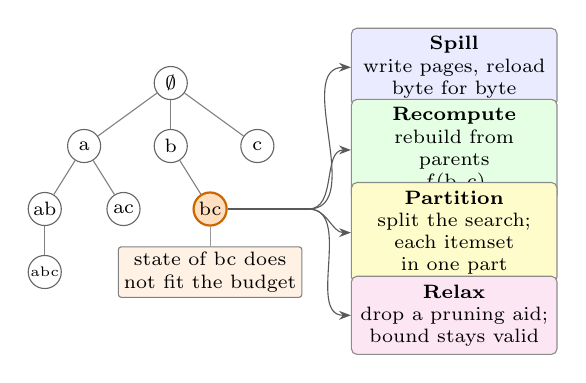
\begin{tikzpicture}[font=\footnotesize,
  nd/.style={circle, draw=black!60, inner sep=0pt, minimum size=4.2mm, font=\scriptsize},
  hot/.style={nd, fill=orange!25, draw=orange!80!black, thick},
  st/.style={draw=black!50, rounded corners=1pt, fill=orange!10, font=\scriptsize, inner sep=2pt},
  mv/.style={draw=black!45, rounded corners=2pt, align=center, text width=24mm, inner sep=3pt, font=\scriptsize},
  arr/.style={-{Stealth[length=1.5mm]}, black!65}]
% search tree
\node[nd] (r) at (0,0) {$\emptyset$};
\node[nd] (a) at (-1.1,-0.8) {a}; \node[nd] (b) at (0,-0.8) {b}; \node[nd] (c) at (1.1,-0.8) {c};
\node[nd] (ab) at (-1.6,-1.6) {ab}; \node[nd] (ac) at (-0.6,-1.6) {ac}; \node[hot] (bc) at (0.5,-1.6) {bc};
\node[nd] (abc) at (-1.6,-2.4) {\tiny abc};
\foreach \u/\v in {r/a,r/b,r/c,a/ab,a/ac,b/bc,ab/abc} \draw[black!50] (\u)--(\v);
\node[st, below=2.5mm of bc, align=center] (state) {state of bc does\\ not fit the budget};
\draw[black!40] (state)--(bc);
\coordinate (j) at (1.75,-1.6);
\draw[black!65, thick] (bc.east)--(j);
\node[mv, fill=blue!8] (sp) at (3.6,0.2) {\textbf{Spill}\\ write pages, reload\\ byte for byte};
\node[mv, fill=green!10] (rc) at (3.6,-0.85) {\textbf{Recompute}\\ rebuild from parents\\ $f(\mathrm{b},\mathrm{c})$};
\node[mv, fill=yellow!20] (pt) at (3.6,-1.9) {\textbf{Partition}\\ split the search;\\ each itemset in one part};
\node[mv, fill=magenta!10] (rx) at (3.6,-2.95) {\textbf{Relax}\\ drop a pruning aid;\\ bound stays valid};
\foreach \m in {sp,rc,pt,rx} \draw[arr] (j) to[out=0,in=180] (\m.west);
\end{tikzpicture}}
\caption{The four moves. When a node's state does not fit, it can be spilled, recomputed from its
parents, avoided by partitioning the search, or, for pruning aids only, relaxed to a looser valid
bound. Each move leaves the set of reported itemsets unchanged.}
\label{fig:moves}
\end{figure}

\setlength{\fboxsep}{1.2pt}
\newcommand{\mS}[1]{\colorbox{blue!8}{S}~#1}
\newcommand{\mR}[1]{\colorbox{green!10}{R}~#1}
\newcommand{\mP}[1]{\colorbox{yellow!20}{P}~#1}
\newcommand{\mX}[1]{\colorbox{magenta!10}{X}~#1}
\begin{table*}[t]
\centering
\caption{The operator matrix: each engine's state and the move applied to it when the budget is
reached. \colorbox{blue!8}{S}\,spill, \colorbox{green!10}{R}\,recompute,
\colorbox{yellow!20}{P}\,partition, \colorbox{magenta!10}{X}\,relax. The last column is the
resident core that admission control requires.}
\label{tab:matrix}
\scriptsize
\setlength{\tabcolsep}{3pt}
\renewcommand{\arraystretch}{1.25}
\begin{tabular}{@{}*{7}{>{\raggedright\arraybackslash}p{2.25cm}}@{}}
\toprule
Engine (algorithms) & Input DB & Base structures & Derived search state & Pruning aids & Candidates & Resident core \\
\midrule
\textbf{Utility lists} (HUI-Miner, FHM, FHM+, HUP-Miner, mHUIMiner, TKO, REPT, HAUI-Miner, HUIM-MMU, IncFHM, SHUIM)
& \mS{filtered DB spool}
& \mS{1-itemset lists by external sort, multi-pass merge}
& \mS{list chunks} or \mR{dropped list rebuilt from parents (cost model)}
& \mP{EUCS built in partitions}; \mX{EUCS disabled, never truncated}
& none
& list headers; one streaming join per worker; top-$k$ heap \\
\textbf{Projection} (EFIM, EFIM-Closed)
& \mS{paged database}
& item renaming (resident)
& \mS{projections as pool pages}; \mP{first-level tasks in batches}
& sub-tree and local utility arrays (resident)
& none
& one projection per worker (two for EFIM-Closed) \\
\textbf{Trees} (IHUP, UP-Growth, UP-Growth+, HUP-Tree, HUI-Trie, TKU)
& \mS{database spool}
& \mP{one small tree per item instead of the global tree}
& \mP{conditional trees inside the item's partition}
& node bounds per partition (valid, at least as tight)
& \mS{spooled}; \mP{verified in bounded rounds}
& TWU map; two node pages; spool buffers \\
\textbf{Two-phase} (Two-Phase)
& \mS{filtered DB spool}
& \mS{1-itemset lists}
& \mS{list chunks}
& TWU only
& \mS{on disk}; \mP{verified in batches}
& list headers; one join per worker \\
\textbf{Heuristics} (HUIM-GA, HUIM-BPSO, MHUI-ACO)
& \mS{DB segments}
& \mS{streamed per selected item}
& population (resident)
& \mX{reported set becomes a Bloom filter (approximate by design)}
& none
& per-item index; one chunk per item \\
\bottomrule
\end{tabular}
\end{table*}

% ---------------------------------------------------------------------------------------------
\section{Architecture}\label{sec:design}

Fig.~\ref{fig:arch} shows how the moves are executed. Engines never allocate growing state
directly: they ask the \emph{state manager} for a reservation, and a refusal is their signal to
apply a move. The state manager owns the ledger, the cost model that chooses between spilling and
recomputing, admission control, and a feedback loop from the real RSS. Below it, one storage layer
serves every engine.

\begin{figure*}[t]
\centering
\resizebox{\textwidth}{!}{%
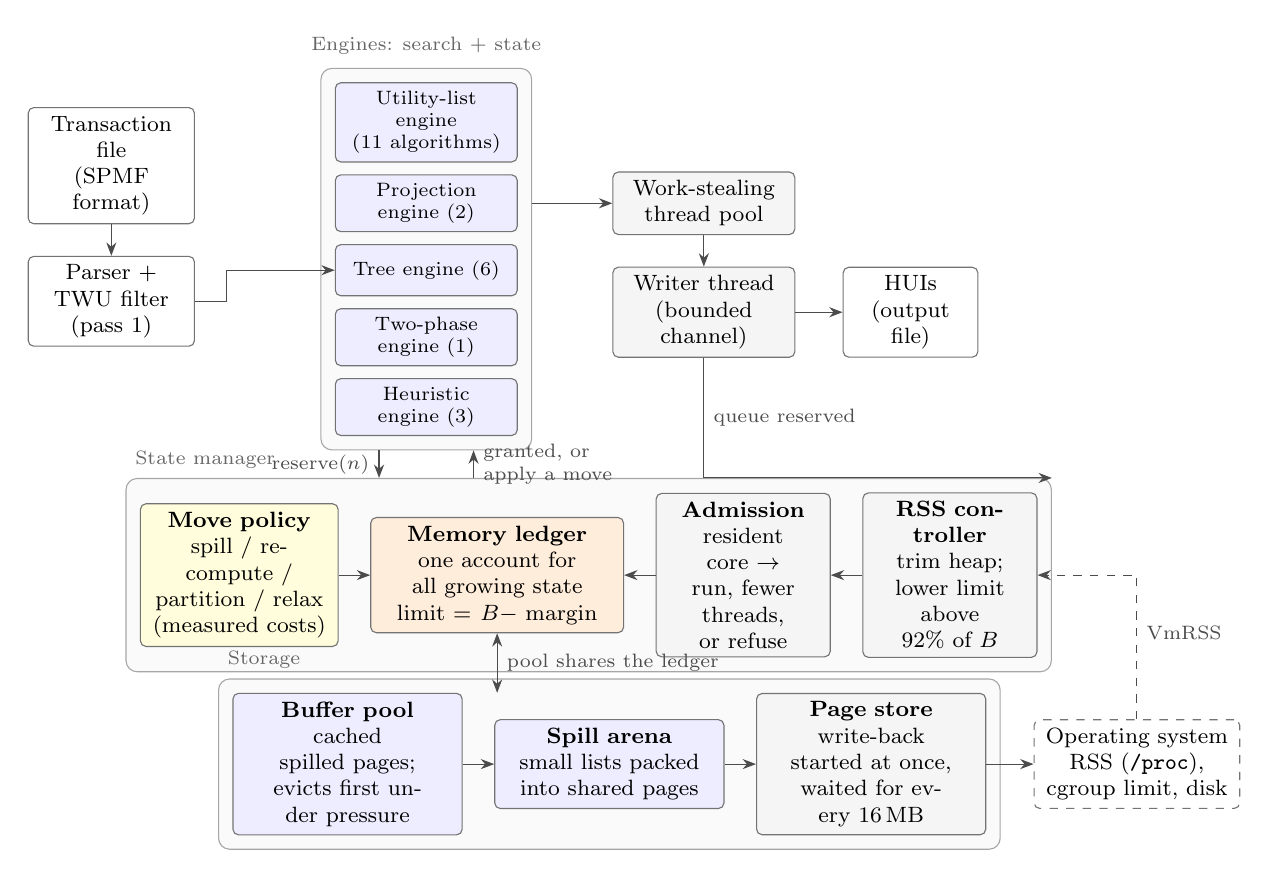
\begin{tikzpicture}[font=\footnotesize, node distance=3mm,
  box/.style={draw=black!55, rounded corners=2pt, align=center, inner sep=3pt, minimum height=7mm},
  eng/.style={box, fill=blue!7, text width=21mm, minimum height=6.5mm, font=\scriptsize},
  lay/.style={draw=black!35, rounded corners=4pt, fill=black!2, inner sep=4pt},
  lab/.style={font=\scriptsize\bfseries, text=black!60, anchor=north west},
  arr/.style={-{Stealth[length=1.7mm]}, black!70},
  dar/.style={{Stealth[length=1.7mm]}-{Stealth[length=1.7mm]}, black!70}]
% input
\node[box, text width=19mm] (file) at (0,0) {Transaction file\\ (SPMF format)};
\node[box, text width=19mm, below=4mm of file] (parse) {Parser + TWU filter\\ (pass 1)};
\draw[arr] (file)--(parse);
% engines
\node[eng] (e1) at (4.0,0.55) {Utility-list engine\\ (11 algorithms)};
\node[eng, below=1.5mm of e1] (e2) {Projection engine (2)};
\node[eng, below=1.5mm of e2] (e3) {Tree engine (6)};
\node[eng, below=1.5mm of e3] (e4) {Two-phase engine (1)};
\node[eng, below=1.5mm of e4] (e5) {Heuristic engine (3)};
\begin{scope}[on background layer]\node[lay, fit=(e1)(e5), inner sep=5pt] (englay) {};\end{scope}

\draw[arr] (parse.east) -- ++(4mm,0) |- (e3.west);
\node[font=\scriptsize, text=black!60, above=0.5mm of englay] {Engines: search + state};
% work-stealing and writer
\node[box, text width=21mm, fill=black!4, right=12mm of e2] (pool) {Work-stealing\\ thread pool};
\node[box, text width=21mm, fill=black!4, below=4mm of pool] (writer) {Writer thread\\ (bounded channel)};
\node[box, text width=15mm, right=6mm of writer] (out) {HUIs\\ (output file)};
\draw[arr] (englay.east |- pool) -- (pool);
\draw[arr] (pool)--(writer); \draw[arr] (writer)--(out);
% state manager
\node[box, fill=orange!14, text width=30mm, minimum height=10mm] (ledger) at (4.9,-5.2) {\textbf{Memory ledger}\\ one account for all growing state\\ limit $= B - $ margin};
\node[box, fill=yellow!14, text width=23mm, left=4mm of ledger] (policy) {\textbf{Move policy}\\ spill / recompute / partition / relax\\ (measured costs)};
\node[box, fill=black!4, text width=20mm, right=4mm of ledger] (adm) {\textbf{Admission}\\ resident core $\to$\\ run, fewer threads, or refuse};
\node[box, fill=black!4, text width=20mm, right=4mm of adm] (rssc) {\textbf{RSS controller}\\ trim heap; lower limit\\ above 92\% of $B$};
\begin{scope}[on background layer]\node[lay, fit=(policy)(rssc), inner sep=5pt] (smlay) {};\end{scope}
\node[font=\scriptsize, text=black!60, anchor=south west] at (smlay.north west) {State manager};
\draw[arr] ([xshift=-6mm]englay.south) -- node[left, font=\scriptsize, align=right]{reserve($n$)} ([xshift=-6mm]smlay.north -| englay.south);
\draw[arr] ([xshift=6mm]smlay.north -| englay.south) -- node[right, font=\scriptsize, align=left]{granted, or\\ apply a move} ([xshift=6mm]englay.south);
\draw[arr] (policy)--(ledger); \draw[arr] (adm)--(ledger); \draw[arr] (rssc)--(adm.east);
\draw[arr] (writer.south) |- node[pos=0.25, right, font=\scriptsize]{queue reserved} (smlay.north east);
% storage
\node[box, fill=blue!7, text width=27mm] (bp) at (3.0,-7.6) {\textbf{Buffer pool}\\ cached spilled pages;\\ evicts first under pressure};
\node[box, fill=blue!7, text width=27mm, right=4mm of bp] (arena) {\textbf{Spill arena}\\ small lists packed\\ into shared pages};
\node[box, fill=black!4, text width=27mm, right=4mm of arena] (store) {\textbf{Page store}\\ write-back started at once,\\ waited for every 16\,MB};
\begin{scope}[on background layer]\node[lay, fit=(bp)(store), inner sep=5pt] (stlay) {};\end{scope}
\node[font=\scriptsize, text=black!60, anchor=south west] at (stlay.north west) {Storage};
\draw[dar] (ledger.south) -- node[right, font=\scriptsize]{pool shares the ledger} (bp.north -| ledger.south);
\draw[arr] (bp)--(arena); \draw[arr] (arena)--(store);
% OS
\node[box, fill=white, text width=24mm, right=6mm of store, dashed] (os) {Operating system\\ RSS (\texttt{/proc}), cgroup limit, disk};
\draw[arr] (store)--(os);
\draw[arr, dashed] (os.north) |- node[pos=0.3, right, font=\scriptsize]{VmRSS} (rssc.east);
\end{tikzpicture}}
\caption{Air-HUIM's architecture. Engines run the search and hold its state, but every byte of state
that grows with the data is reserved from the state manager first; a refused reservation makes the
engine apply one of the four moves. The buffer pool shares the same ledger, admission control sizes
the resident core before mining, and the RSS controller corrects the ledger with the memory the
process really uses.}
\label{fig:arch}
\end{figure*}

\textbf{The budget.} The user passes one number $B$ (e.g.\ \texttt{-b 64} for 64\,MB). The goal
is that the process RSS stays within $B$, that the run uses $B$ (data stays in RAM while it fits),
and that the output is identical at every $B$.

\textbf{One ledger.} A single \texttt{MemoryGuard} accounts for everything that grows with the data:
native structures (utility lists, projections, trees, the pair-utility matrix, the top-$k$ heap)
through RAII reservations released when the structure is dropped; buffer-pool frames, which the
pool charges when it caches a page; and the process baseline, read once from \texttt{VmRSS}. The
ledger's limit is $B$ minus a margin of 7\,MB\,+\,3\% (at most 128\,MB and at most $B/2$) for what it
cannot see: allocator metadata, I/O buffers and thread stacks. A reservation either succeeds or
tells the caller to fall back (spill, recompute or partition); small bounded buffers use a forced
reservation that is accounted but never refused.

\textbf{Buffer pool and spill.} Spilled data lives in a page store on disk behind a buffer pool that
shares the ledger. Cached pages are copies of spilled data, so when a native reservation fails the
pool evicts first. Pages of dead search branches are discarded without being written. Small spilled
lists are packed into shared pages so that a starved search does not create one file per list.

\textbf{Admission control.} After its first pass, each engine estimates the memory it cannot spill,
as a fixed part plus a per-worker part. If one worker does not fit, the run stops at once with the
smallest workable budget (``Use at least \texttt{-b} 33''); otherwise the thread count is lowered
until the per-worker sets use at most half of the free budget.

\textbf{RSS feedback.} The ledger sees allocations, not resident pages: freed memory that the
allocator keeps, and fragmentation between long- and short-lived blocks, raise RSS above the ledger.
A background thread reads RSS every 250\,ms, returns free heap pages to the OS
(\texttt{malloc\_trim}), and lowers the ledger limit by any excess over 92\% of $B$ (never below
half its starting value), raising it again when RSS falls.

\textbf{Dirty pages.} Under a kernel memory limit (Linux cgroups), dirty page-cache pages count
against the process. Spill writes therefore start write-back immediately and wait for it every
16\,MB, so a burst of spilling cannot push the process over a hard limit.

\textbf{Threads.} The top-level search is split into tasks run by a work-stealing pool; results go
to one writer thread over a bounded channel whose capacity is reserved from the ledger, so a slow
disk applies backpressure instead of growing memory.

% ---------------------------------------------------------------------------------------------
\section{Applying the Moves to Each Engine}\label{sec:model}

This section explains the non-obvious entries of Table~\ref{tab:matrix}.

\textbf{Utility-list engine.} A list body longer than one chunk (4,096 entries, smaller under tiny
budgets) is a sequence of chunks; a join reads the prefix list and the two extension lists one
chunk at a time and writes the result chunk by chunk, so its working set is constant in the list
lengths. When a new list does not fit, a cost model chooses between writing it to disk and
dropping it: a dropped list keeps a recipe and is recomputed from its parents, which are alive
higher up the search, when it is next needed. Costs are measured during the run. The extension
items carry only their last item; the prefix is passed down the search, so no itemset is copied
per extension. EUCS~\cite{fhm2014} is stored as a dense triangular matrix of saturating 32-bit
cells when it fits (a saturated cell never prunes) and otherwise in hashed partitions; it is never
truncated, because a truncated EUCS silently drops valid itemsets.

\textbf{Projection engine.} The database and every projection live in pool pages when they do not
fit; EFIM's transaction merging works on the same pages. EFIM-Closed keeps a spilled projection
and the projection of its child resident at the same time, hence two per worker.

\textbf{Tree engine.} A spilled prefix tree is mined one node-link step at a time, and each step
can be a page load: UP-Growth+ on retail at 32\,MB read 207\,GB of pages for a 26\,MB tree. When the
tree's size bound (one node per item occurrence) exceeds the free budget, the miners switch to
partition projection: each transaction is written to the partition of its last item; items are
processed from the bottom of the order up, each with a small tree built in RAM and mined with the
unchanged per-item code; then each row moves to the partition of its new last item. All disk access
is sequential. Candidate itemsets are spooled to disk and verified, then cleared, whenever the spool
reaches a bounded size, instead of all at the end.

\textbf{Resulting bound.} If the ledger stays within $B$ minus the margin, and the margin covers
what the ledger cannot see, the RSS stays within $B$. The first condition holds by construction:
every growing structure is reserved before it is allocated. The second is empirical. We calibrated
the margin on chainstore (RSS exceeds the ledger peak by about 6.5\,MB at 24--64\,MB budgets and
about 30\,MB at 1\,GB) and check it on every run (Section~\ref{sec:budget}).

% ---------------------------------------------------------------------------------------------
\section{Evaluation}\label{sec:eval}

\subsection{Setup}

\textbf{Hardware.} Raspberry Pi~4 Model~B, 4\,GB RAM, quad-core Cortex-A72 at 1.8\,GHz, 64\,GB SD
card, Debian~13, Linux~6.18. CPU frequency stayed at 1.8\,GHz with no throttling in any run.
Speed comparisons at one thread each, and thread scaling beyond four threads, were run on a laptop
(AMD Ryzen~7 7435HS, 8 cores and 16 threads, 23\,GB RAM; Section~\ref{sec:speed}).

\textbf{Software.} Air-HUIM built with Rust~1.99 in release mode. SPMF~2.67a~\cite{spmf2016} on
OpenJDK~25 with \texttt{-Xmx} set to the budget. Both read the same files (checksums recorded per
run) with the same thresholds.

\textbf{Datasets.} Table~\ref{tab:data} lists the 14 standard benchmark datasets and LGSR, a
simulated but realistic retail dataset from dunnhumby~\cite{lgsr}, converted to 47.1\,M baskets
(3.4\,GB in SPMF format).

\begin{table}[t]
\centering
\caption{Datasets and thresholds (\% of total utility).}
\label{tab:data}
\footnotesize
\begin{tabular}{@{}lrrrr@{}}
\toprule
Dataset & Transactions & Items & Avg.\ length & min\_util (\%) \\
\midrule
foodmart & 4,141 & 1,559 & 4.4 & 0.025 \\
chess & 3,196 & 75 & 37.0 & 25 \\
mushroom & 8,124 & 119 & 23.0 & 5 \\
ecommerce & 14,975 & 3,468 & 11.6 & 0.2 \\
pumsb & 49,046 & 2,113 & 74.0 & 23 \\
liquor & 52,131 & 4,026 & 7.9 & 0.005 \\
BMS & 59,602 & 497 & 2.5 & 2.1 \\
connect & 67,557 & 129 & 43.0 & 32 \\
retail & 88,162 & 16,470 & 10.3 & 0.01 \\
fruithut & 181,970 & 1,265 & 3.6 & 0.01 \\
accidents & 340,183 & 468 & 33.8 & 12 \\
kosarak & 990,002 & 41,270 & 8.1 & 1 \\
chainstore & 1,112,949 & 46,086 & 7.2 & 0.1 \\
chicago & 2,662,309 & 35 & 1.8 & 0.005 \\
LGSR & 47,098,416 & 4,997 & 6.5 & 0.2 \\
\bottomrule
\end{tabular}
\end{table}

\textbf{Protocol.} A harness runs one job at a time, samples RSS every 100\,ms,
and records status, wall time, peak RSS, the binary's hash and the dataset's checksum. Runs are
capped at 10\,min (LGSR: 4\,h). Exactness is checked against a reference output computed by
Air-HUIM FHM at a large budget; every disagreement between implementations is settled by a full
scan of the dataset (Section~\ref{sec:spmf}). A run is \emph{out of memory} when the JVM reports
it, or when the kernel limit or the watchdog kills it.

\subsection{Exactness}

All 905 Air-HUIM runs with a reference output matched it exactly, at every budget and thread
count. Top-$k$ and REPT runs have no fixed reference; a full scan confirmed every utility in the
top-$k$ outputs on every dataset. The three metaheuristics are approximate by design and excluded.

\subsection{Budget adherence}\label{sec:budget}

Of 1,503 Air-HUIM runs, 1,489 peaked at or below the budget. Thirteen exceeded it by 0.1--3.2\,MB,
all at 24--64\,MB; the fourteenth, EFIM-Closed on LGSR at 2\,GB, peaked at 2,075\,MB (+1.3\%).
Fig.~\ref{fig:peak} compares peak memory with the budget for every comparison run: SPMF's JVM
exceeds a 64\,MB heap budget in every run, by up to $2.6\times$. Table~\ref{tab:hard} shows both tools under two hard limits: a kernel-enforced cgroup memory limit,
and a watchdog that kills any process whose RSS exceeds the budget.

\begin{table}[t]
\centering
\caption{Runs killed under hard memory limits (Raspberry Pi).}
\label{tab:hard}
\footnotesize
\begin{tabular}{@{}lccc@{}}
\toprule
Limit & Budgets & Air-HUIM killed & SPMF killed \\
\midrule
cgroup \texttt{MemoryMax} & 64--256\,MB & 0 / 90 & 72 / 90 \\
Watchdog (RSS $>$ budget) & 64--256\,MB & 0 / 32 & 32 / 32 \\
\bottomrule
\end{tabular}
\end{table}

\begin{figure}[t]
\centering
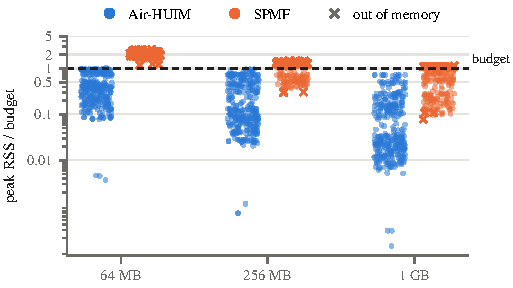
\includegraphics[width=\columnwidth]{fig/peak_ratio.pdf}
\caption{Peak RSS divided by the budget, every Air-HUIM and SPMF run of the comparison (Pi, log
scale). Crosses are runs that ran out of memory. SPMF's heap limit does not bound the process:
the JVM's own memory comes on top.}
\label{fig:peak}
\end{figure}

\subsection{Air-HUIM versus SPMF at the same budget}

For every algorithm both libraries implement, we ran both on each dataset at 64\,MB, 256\,MB and
1\,GB: 196 pairs per budget. Fig.~\ref{fig:outcomes} counts the outcomes.

\begin{figure}[t]
\centering
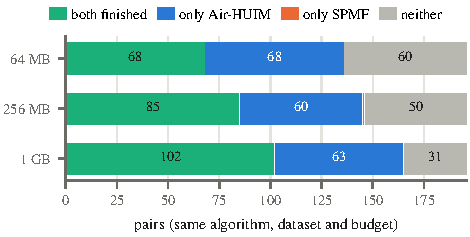
\includegraphics[width=\columnwidth]{fig/outcomes.pdf}
\caption{Outcome of the 196 Air-HUIM/SPMF pairs at each budget on the Pi (same algorithm, dataset
and budget; 10\,min cap). Only SPMF finished in one pair, at 256\,MB.}
\label{fig:outcomes}
\end{figure}


At 64\,MB, only Air-HUIM finished in 68 pairs and only SPMF in none. Where neither finished,
Air-HUIM hit the time cap without running out of memory; SPMF ran out of memory in 56 of those 60
pairs at 64\,MB. In total SPMF ran out of memory in 116, 79 and 34 pairs at 64\,MB, 256\,MB
and 1\,GB.

\subsection{Graceful degradation}

Fig.~\ref{fig:curve} shows Air-HUIM's run time as the budget shrinks from 2\,GB to 32\,MB. Above
the size of the working set, time is flat. Below it, time rises smoothly as more state is spilled
or recomputed; there is no cliff where a run fails, and the output is identical at every budget.
Two-Phase does not finish on accidents, kosarak and retail at any budget: its candidate set is too
large at these thresholds, independent of memory.

\begin{figure*}[t]
\centering
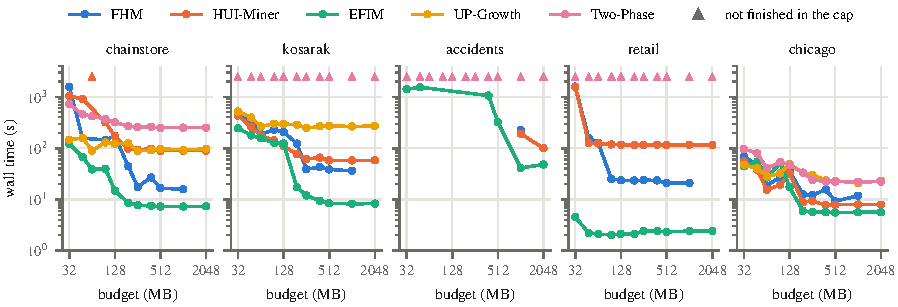
\includegraphics[width=\textwidth]{fig/budget_curve.pdf}
\caption{Air-HUIM wall time against budget on the Pi (4 threads, log--log). Lines join finished
runs; triangles mark budgets where a run reached its time cap (10 or 30\,min). Output is identical
at every budget.}
\label{fig:curve}
\end{figure*}

\subsection{47 million baskets on a Raspberry Pi}

Fig.~\ref{fig:lgsr} shows LGSR on the Pi at 1 and 2\,GB, with 4 threads for Air-HUIM. SPMF ran out
of memory in all 8 runs, after 1--13 minutes. Air-HUIM finished 7 of 8 with the exact 52 HUIs;
EFIM-Closed at 1\,GB reached the 4-hour cap without exceeding its budget. Air-HUIM's peaks were
894--1,982\,MB for FHM, EFIM and EFIM-Closed, all within budget except EFIM-Closed at 2\,GB
(2,075\,MB).

\begin{figure}[t]
\centering
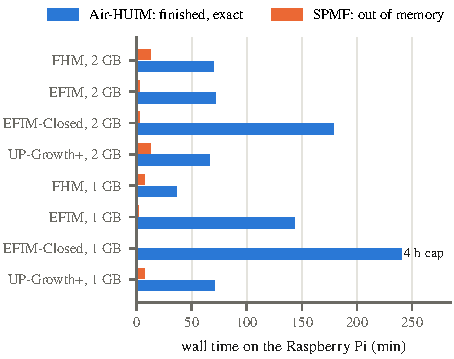
\includegraphics[width=\columnwidth]{fig/lgsr.pdf}
\caption{LGSR (47.1\,M baskets, min\_util 0.2\%) on the 4\,GB Raspberry Pi: time until SPMF ran
out of memory, and time until Air-HUIM finished.}
\label{fig:lgsr}
\end{figure}


UP-Growth+ needs about 100\,MB at either budget: partition projection keeps only one item's
tree in memory at a time.

\subsection{Speed at one thread each}\label{sec:speed}

SPMF is single-threaded, so we compare one thread against one thread on a laptop, repeating each
of the 102 pairs that both libraries finished at 1\,GB on the Pi five times and reporting the
median (Fig.~\ref{fig:speed}). Wall time includes process start-up, which costs SPMF about
0.5\,s for the JVM. Air-HUIM is faster on 63 of the 102 pairs, with a median speed-up of
1.37$\times$. Counting only the 74 pairs where both tools take at least a second, the two are
level: the median is 1.07$\times$, and Air-HUIM is faster on 38.

The spread is wide. EFIM is 17--27$\times$ faster on connect, pumsb and liquor, and TKO is
32$\times$ faster on retail. In the other direction, EFIM-Closed and TKU on mushroom are 17$\times$
and 11$\times$ slower, and the utility-list miners on the sparse retail, liquor and fruithut sets
are about 3$\times$ slower. Budget safety is therefore not free in every case. We have not yet
profiled these slow cases.

\begin{figure}[t]
\centering
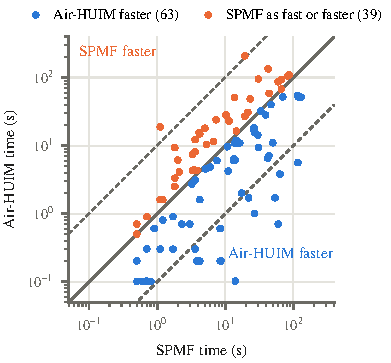
\includegraphics[width=\columnwidth]{fig/speed.pdf}
\caption{One thread against one thread: median of five runs for each of the 102 pairs both
libraries finished, 1\,GB budget, laptop. Solid line: equal time; dashed lines: 10$\times$
either way.}
\label{fig:speed}
\end{figure}

\subsection{Thread scaling}

Fig.~\ref{fig:threads} shows Air-HUIM on the Pi with 1, 2 and 4 threads at 1\,GB. Speed-ups from
1 to 4 threads range from 1.1$\times$ to 3.7$\times$ (median 1.8$\times$). Short runs (EFIM on
chainstore and kosarak, under 12\,s) are dominated by reading the input, which is sequential. FHM
and HUI-Miner on accidents are slower at 4 threads than at 2. \pending{laptop 1--16 threads on
LGSR, chainstore$\times$40 and H\&M; queued after the 1-thread table}

\begin{figure}[t]
\centering
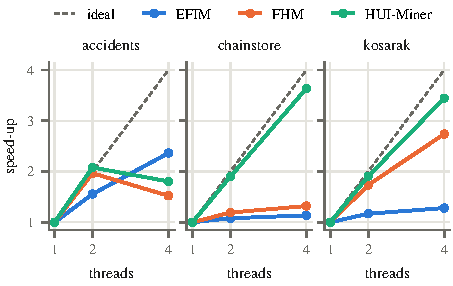
\includegraphics[width=\columnwidth]{fig/threads_pi.pdf}
\caption{Speed-up over one thread on the 4-core Pi (1\,GB budget). HUI-Miner scales best; EFIM's
short runs are dominated by sequential input reading.}
\label{fig:threads}
\end{figure}


% ---------------------------------------------------------------------------------------------
\section{Correctness Problems Found in SPMF}\label{sec:spmf}

Every itemset on which SPMF and Air-HUIM disagreed was settled by computing its exact utility in a
plain scan of the dataset, independent of both libraries. Air-HUIM's output was exact in every
comparison. SPMF showed three problems (Table~\ref{tab:spmf}).

\begin{table}[t]
\centering
\caption{Correctness problems in SPMF 2.67a.}
\label{tab:spmf}
\footnotesize
\begin{tabular}{@{}p{1.4cm}p{2.9cm}p{3.6cm}@{}}
\toprule
Algorithm & Problem & Effect \\
\midrule
FHM, FHM+ & item comparator casts the 64-bit TWU difference to a 32-bit \texttt{int} & once TWUs differ by $2^{31}$, the order is inconsistent; on LGSR 20,134 of 1.52\,M item pairs are misordered and one true HUI is missed \\
mHUIMiner & item labels in the output are corrupted & correct count, wrong itemsets on 10 of 12 datasets (retail: 16,308 of 22,479) \\
TKU & returns fewer than $k$ itemsets & on chicago with $k=100$ it returns 4; SPMF's own TKO returns 100 \\
\bottomrule
\end{tabular}
\end{table}

The FHM problem was confirmed in the bytecode (\texttt{lsub} followed by \texttt{l2i}); it did not
appear on the 14 benchmark datasets, but appears on retail data with billions in total utility. The TKU problem reproduces with a 1\,GB and a 4\,GB heap, so it is
not a memory effect.

% ---------------------------------------------------------------------------------------------
\section{Limitations}

The budget is not yet a strict ceiling: 14 of 1,503 runs exceeded it, by at most 3.2\,MB at small
budgets and by 1.3\% for EFIM-Closed on LGSR; we have not yet found the allocation the ledger
misses. Some algorithms are slow at small budgets for reasons unrelated to memory (TWU-only bounds
give too many candidates for IHUP, HUI-Trie and HUP-Tree on retail and kosarak). The Pi
experiments ran each configuration once; the speed comparison uses five repeats. LGSR is simulated
retail data.

\section{Conclusion}

Air-HUIM shows that the standard HUIM algorithms can run exactly under a hard memory budget on a
4\,GB single-board computer, including on 47 million baskets, where the reference implementation
fails. The method is uniform across 23 algorithms: one ledger, spill or recompute or partition, and
clean refusal below a computed minimum. The library, benchmark harness and all run records are
available at \url{https://github.com/CyberKnight-cmd/pocket-data-mining} and archived as release 1.0.0 at
\url{https://doi.org/10.5281/zenodo.24039625}.

\bibliographystyle{IEEEtran}
\bibliography{refs}

\end{document}
